\documentclass[11pt]{article}
\usepackage{theme}
\usepackage{shortcuts}
\usepackage{algorithm}
\usepackage[noend]{algpseudocode}
\usepackage{amsmath}
\newcommand{\jump}{\newline\newline}
% Document parameters
% Document title 
\title{Detecting Changes in Slope With an $L_0$ Penalty}
\author{
Bastien LE CHENADEC \email{bastien.le-chenadec@eleves.enpc.fr} \\ % student 1
Sofiane EZZEHI \email{sofiane.ezzehi@eleves.enpc.fr} % student 2
}

\begin{document}
\maketitle
\paragraph{What is expected for these mini-projects?}
\textit{
    The goal of the exercise is to read (and understand) a research article, implement it (or find an implementation), test it on real data and comment on the results obtained.
    Depending on the articles, the task will not always be the same: some articles are more theoretical or complex, others are in the direct line of the course, etc... It is therefore important to balance the exercise according to the article. For example, if you have reused an existing implementation, it is obvious that you will have to develop in a more detailed way the analysis of the results, the influence of the parameters etc... Do not hesitate to contact us by email if you wish to be guided.}

\paragraph{The report}
\textit{
    The report must be at most FIVE pages and use this template (excluding references). If needed, additional images and tables can be put in Appendix, but must be discussed in the main document. The report must contain a precise description of the work done, a description of the method, and the results of your tests. Please do not include source code! The report must clearly show the elements that you have done yourself and those that you have reused only, as well as the distribution of tasks within the team (see detailed plan below.)}

\paragraph{The source code}
\textit{
    In addition to this report, you will have to send us a Python notebook allowing to launch the code and to test it on data. For the data, you can find it on standard sites like Kaggle, or the site https://timeseriesclassification.com/ which contains a lot of signals!}


\paragraph{The oral presentations}
\textit{
    They will last 10 minutes followed by 5 minutes of questions. The plan of the defense is the same as the one of the report: presentation of the work done, description of the method and analysis of the results.}


\paragraph{Deadlines}
\textit{
    Two sessions will be available :
    \begin{itemize}
        \item \textbf{Session 1}
              \begin{itemize}
                  \item Deadline for report: December 18th (23:59)
                  \item Oral presentations: December 20th and 22th (precise times TBA)
              \end{itemize}
        \item \textbf{Session 2}
              \begin{itemize}
                  \item Deadline for report: January 9th (23:59)
                  \item Oral presentations: January, 11th and 12th (precise times TBA)
              \end{itemize}
    \end{itemize}}

\section{Introduction and contributions}

\textit{
    The Introduction section (indicative length : less than 1 page) should detail the scientific context of the article you chose, as well as the task that you want to solve (especially if you apply it on novel data). \textbf{The last paragraph of the introduction must contain the following information}:
    \begin{itemize}
        \item Repartition of work between the two students
        \item Use of available source code or not, percentage of the source code that has been reused, etc.
        \item Use of existing experiments or new experiments (e.g. test of the influence of parameter that was not conducted in the original article, application of the method on a novel task/data set etc.)
        \item Improvement on the original method (e.g. new pre/post processing steps, grid search for optimal parameters etc.)
    \end{itemize}
}

\section{Method}

\textit{
    The Method section (indicative length : 1 to 2 pages) should describe the mathematical aspects of the method in a summarized manner. Only the main steps that are useful for understanding should be highlighted. If relevant, some details on implementation can be provided (but only marginally).
}

A word on notations : if we have a sequence $x=x_1,\dots,x_n$, we denote $x[s:t]$ the subsequence $x_s,\dots,x_t$.

\subsection{Model}

Let $y=y_1, \dots, y_n$ be successive data points in time. The goal of this method is to find $m$ changepoints $\tau_1,\dots,\tau_m$ such that the data is divided in $m+1$ segments. We let $\tau_0=0$ and $\tau_{m+1}=n$; the segment $j$ is then $y_{\tau_{j-1}+1},\dots,y_{\tau_j}$.

The method considers a piecewise linear model to fit the data. We denote $\phi_{\tau_j}$ the value taken by the model at time $\tau_j$. Under these assumptions, the model writes :
\begin{equation}
    \forall 0\leq i\leq m,\,\forall \tau_i+1\leq t\leq \tau_{i+1},\quad Y_t=\phi_{\tau_i}+\frac{\phi_{\tau_{i+1}}-\phi_{\tau_i}}{\tau_{i+1}-\tau_i}(t-\tau_i)+Z_t
\end{equation}
where $(Z_t)_{1\leq t\leq n}$ is assumed to be a gaussian white noise with variance $\sigma^2$.

\subsection{Penalized cost approach}

The method uses a penalized cost approach to find the changepoints. The cost function is a squarred error loss, penalized by a term that depends on the segments length, and an $L_0$ penalty on the number of changepoints. The cost function naturally writes :
\begin{equation}
    \sum_{i=0}^m \left[\frac{1}{\sigma^2}\sum_{t=\tau_i+1}^{\tau_{i+1}} \left(y_t-\phi_{\tau_i}-\frac{\phi_{\tau_{i+1}}-\phi_{\tau_i}}{\tau_{i+1}-\tau_i}(t-\tau_i)\right)^2 + h(\tau_{i+1}-\tau_i)\right]+\beta m
\end{equation}
By introducing a segment cost, for fitting a segment that takes the value $\phi$ at time $s$ and $\psi$ at time $t$, on the data $y_{s+1},\dots,y_t$, that writes :
\begin{equation}
    \mathcal{C}(y[s+1:t],\phi,\psi) = \frac{1}{\sigma^2}\sum_{j=s+1}^t \left(y_j-\phi-\frac{\psi-\phi}{t-s}(j-s)\right)^2
\end{equation}

the penalized cost function can be rewritten as :
\begin{equation}
    \label{eq:problem}
    \min_{\substack{m\\\tau_1,\dots,\tau_m\\ \phi_0,\dots,\phi_{m+1}}} \beta m+\sum_{i=0}^m \mathcal{C}(y[\tau_i+1:\tau_{i+1}],\phi_{\tau_i},\phi_{\tau_{i+1}}) + h(\tau_{i+1}-\tau_i)
\end{equation}

\subsection{Dynamic programming}

We want to solve the problem \eqref{eq:problem} by dynamic programming. Compared to other changepoints detection methods, the difficulty lies in the continuity constraint between segments. Thus the authors introduce $f^t(\phi)$ as the minimum cost for segmenting $y_1,\dots,y_t$ in $k+1$ segments conditionally on the model taking the value $\phi$ at time $t$ :
\begin{equation}
    \begin{aligned}
        f^t(\phi)=\min_{\substack{\tau_1,\dots,\tau_{k}                         \\ \phi_0,\dots,\phi_k}} &\sum_{i=0}^{k-1} \mathcal{C}(y[\tau_i+1:\tau_{i+1}],\phi_{\tau_i},\phi_{\tau_{i+1}}) + h(\tau_{i+1}-\tau_i)\\
         & +\mathcal{C}(y[\tau_k+1:t],\phi_{\tau_k},\phi)+h(t-\tau_k) + \beta k
    \end{aligned}
\end{equation}
which they are able to express recursively :
\begin{equation}
    f^t(\phi)=\min_{\phi',s} f^s(\phi')+\mathcal{C}(y[s+1:t],\phi',\phi)+h(t-s)+\beta
\end{equation}

They also introduce $f^t_{\boldsymbol{\tau}}(\phi)$ which is the minimum cost for segmenting $y_1,\dots,y_t$ in $k+1$ segments conditionally on the model taking the value $\phi$ at time $t$ and the changepoints being $\boldsymbol{\tau}=(\tau_0,\tau_1,\dots,\tau_k,\tau_{k+1})$. This quantity is a quadratic polynomial in $\phi$ and the authors are able to express its coefficients recursively. All of this allows them to compute $f^n(\phi)$ in $\mathcal{O}(n!/(n-m)!)$.

\subsection{Pruning}

Given the high complexity of the dynamic programming algorithm (exploring the space of all possible changepoints), the authors introduce multiple pruning techniques to reduce the complexity.

\paragraph*{Functional pruning} The authors introduce $\mathcal{T}_t$ the set of all possible changepoint vectors at time $t$, and $\mathcal{T}_t^*=\left\{\boldsymbol{\tau}\in \mathcal{T}_t \:\big|\: \exists\phi\in\mathbb{R}, f^t(\phi)=f_{\boldsymbol{\tau}}^t(\phi)\right\}$ the set of changepoint vectors at time $t$ that are optimal for some $\phi$.

\begin{theorem}
    \label{th:functional_pruning}
    Let $\boldsymbol{\tau}\in\mathcal{T}_s$ such that $\boldsymbol{\tau}\notin \mathcal{T}_s^*$. Then $\boldsymbol{\tau}\notin \mathcal{T}_t^*$ for all $t>s$.
\end{theorem}

This theorem allows us to only explore $\hat{\mathcal{T}}_t=\left\{(\boldsymbol{\tau},s)\:\big|\: 0\leq s\leq t-1, \boldsymbol{\tau}\in \mathcal{T}_s^*\right\}$ when computing $f^t(\phi)$.

\paragraph*{Inequality based pruning} Let $K=2\beta+h(1)+h(n)$. Suppose that $h$ is non-negative and non-decreasing.

\begin{theorem}
    Let $\tau\in\mathcal{T}_s$ such that :
    $$\min_\phi f_{\boldsymbol{\tau}}^s(\phi) > K + \min_{\phi'} f^s(\phi')$$
    Then $\boldsymbol{\tau}\notin \mathcal{T}_t^*$ for all $t>s$.
\end{theorem}

This theorem allows to further prune the set $\hat{\mathcal{T}}_t$.

\subsection{Algorithm}

The two difficulties of the implementation are storing the coefficients of the polynomials $f^t_{\boldsymbol{\tau}}(\phi)$, and implementing the pruning techniques. The authors provided relatively detailed pseudo-code for the algorithm, but we still found it difficult to implement.

The goal of this first algorithm is to only keep segmentations that are optimal for some values of $\phi$. Segmentation costs are polynomials, so this algorithm starts from the optimum segmentation for $\phi=-\infty$ and iteratively finds the next optimum segmentation by looking at the points where the polynoms intersect.
\begin{algorithm}[H]
    \caption{Functional pruning algorithm}
    \begin{algorithmic}[1]
        \State \textbf{Input:} Candidate segmentations $\hat{\mathcal{T}}_{t}$, costs $f^{t}_{{\tau}}(\phi)$ for ${\tau}\in\hat{\mathcal{T}}_{t}$.

        \State \textbf{Initialize:} $\phi_\text{curr}=-\infty \quad {\tau}_{curr}=\underset{{\tau}\in\hat{\mathcal{T}}_{t}}{ \arg\min}\left[f^{t}_{{\tau}}(\phi_{curr})\right]\quad \mathcal{T}_{temp}=\hat{\mathcal{T}}_{t}\setminus \left\{\tau_{curr}\right\}\quad \mathcal{T}^*_t=\left\{\tau_{curr}\right\}$

        \While{$\mathcal{T}_{temp}\neq\emptyset$}

        \For{$\tau\in\mathcal{T}_{temp}$}
        \State $x_{\tau}=\min\left\{\phi:f^{t}_{\tau}(\phi)-f^{t}_{{\tau}_{curr}}(\phi)=0\;\;\&\;\;\phi>\phi_{curr}\right\}$
        \If {$x_{\tau}=\emptyset$}
        \State $\mathcal{T}_{temp}=\mathcal{T}_{temp}\setminus\left\{\tau\right\}$
        \EndIf
        \EndFor

        \State $\tau_{curr}=\underset{\tau\in\mathcal{T}_{temp}}{\arg\min}(x_{\tau})$
        \State $\phi_{curr}=x_{\tau_{curr}}$
        \State $\mathcal{T}^*_t=\mathcal{T}^*_t\cup\left\{\tau_{curr}\right\}$
        \EndWhile

        \State \textbf{Output:} $\mathcal{T}^*_t$
    \end{algorithmic}
\end{algorithm}

Then we can define the full algorithm that uses both pruning techniques.
\begin{algorithm}[H]
    \caption{CPOP}
    \begin{algorithmic}[1]
        \State \textbf{Input:} Data $y=y_1,\dots,y_n$, penalty $\beta$ and segment cost $h$.

        \State \textbf{Initialize:} $\hat{\mathcal{T}}_1=\left\{\left\{0\right\}\right\}$

        \For {$t=1,\dots,n$} \Comment{Cost computation}
        \For {$\tau\in\hat{\mathcal{T}}_t$}
        \If {$\tau = \left\{0\right\}$}\Comment{No changepoint}
        \State $f^t_{\tau}(\phi)=\min_{\phi'}\mathcal{C}(y[1:t],\phi',\phi)+h(t)$
        \Else \Comment{Compute recursively}
        \State $f^t_{\tau}(\phi)=\min_{\phi'}\left(f^{\tau_k}_{\tau_1,\dots,\tau_{k-1}}(\phi')+\mathcal{C}(y[\tau_k+1:t],\phi',\phi)+h(t-\tau_k)+\beta\right)$
        \EndIf
        \EndFor

        \State $\mathcal{T}^*_t = \text{functional\_pruning}(\hat{\mathcal{T}}_t, f^t)$

        \State $\hat{\mathcal{T}}_{t+1}= \left\{\tau\in \hat{\mathcal{T}}_t \big| \min_\phi f_\tau^t(\phi)\leq \min_{\phi',\tau'}f_{\tau'}^t(\phi')+K\right\}\cup \left\{(\tau, t)\big|\tau\in \mathcal{T}^*_t\right\}$
        \EndFor

        \State \textbf{Output:} $\argmin_{\tau\in \hat{\mathcal{T}}_n}[\min_\phi f^n_\tau(\phi)]$
    \end{algorithmic}
\end{algorithm}
We note that we only need to store the coefficients for $f^{\tau_k}_{\tau_1,\dots,\tau_{k-1}}$.

\section{Data}
\subsection{Data description : Tunisian stock market}
Financial data, and more specifically stock prices across time, are a good candidate to test the method. Indeed, stock prices, taken at a relatively low frequency (daily) are known to exhibit clear trends, while being noisy enough to make the detection of changepoints interesting. And since the method is designed to detect changepoints in a piecewise linear model, it is well suited for this kind of data.
\jump
We test the method on the stock prices of all the listed companies on the Bourse de Tunis, which is Tunisia stock exchange. The data was taken from Kagglee, and is available at \url{https://www.kaggle.com/datasets/amariaziz/tunisian-stock-market}. It contains the Open, High, Low and Close prices of 88 companies, as well as the volume of transactions. We only use the Close prices, which are the prices at the end of the trading day.
\subsection{Data preprocessing}
Since the data was partially collected by web scraping, it naturally requires some cleaning and preprocessing. We detail here the steps we took to clean the data. We are left with $85$ companies.
\paragraph*{Stocks with too few data points} We see on figure \ref{fig:histogram_size} that the number of data points per company is very variable. We remove the stocks that have less than $200$ data points, since they are not interesting for our analysis.
\paragraph*{Missing values and duplicates} Missing values are days where we have corrupted data for a given stock. We see in table \ref{tab:missing_values} that the data is relatively clean of missing values, with only $3$ companies having no more than a few percent of missing values. We see on figure \ref{fig:bar_duplicates} that each stock has between $1\%$ and $3\%$ of duplicates. We remove the missing values as well as the duplicates.
\paragraph*{Missing days} Missing days are days where we have no data at all for a given stock. We see on figure \ref{fig:bar_missing_days} that the number of missing days is clearly the biggest issue with the data, with most stocks having more than $40\%$ of missing days. We deal with this issue by interpolating the missing days, using a linear interpolation between the last and next available data points. We note that this is not a perfect solution, since it assumes that the stock price evolves linearly between two days, which is never the case for stock prices. However, it is a simple solution that allows us to keep the data for all the stocks.
\paragraph*{Data shrinkage by sub-sampling} Since our method is relatively slow for time series longer than a few thousand points, and since our available computational power is limited, we sub-sample the data to reduce its size. We sub-sample the data by only keeping at most $1000$ points per stock, by sampling uniformly on the time axis. We see on figure \ref{fig:subsample} that this sub-sampling very slightly affects the data.
\section{Results}
We present here a few experiments that we conducted on the $85$ Tunisian stocks we preprocessed. First, we zoom on a few stocks to see how the method behaves and we qualitatively compare it to a best-fitting piecewise constant mean model. Second, we investigate the influence of the penalty parameter $\beta$ on the number of changepoints detected. Third, we investigate the influence of the segment cost $h$ on the number of changepoints detected. Finally, we briefly discuss the computational complexity of the method.
\subsection{Qualitative comparison with a piecewise constant mean model}
We compare the method to a piecewise constant mean model, which is the simplest model that can be used to detect changepoints. We note that the nature of the data (stock prices) puts the piecewise constant mean model at a great disadvantage, since stock prices are known to exhibit piecewise linear trends. We only perform this comparison qualitatively.
\begin{figure}[h]
    \centering
    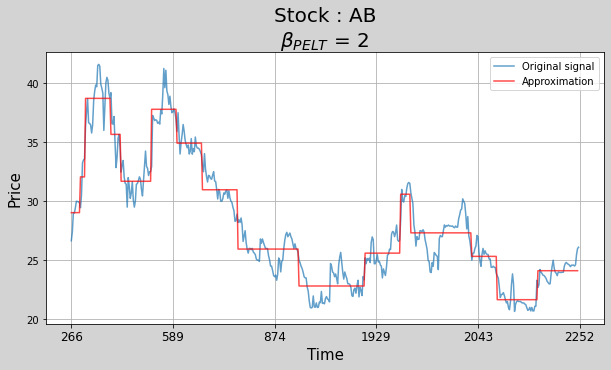
\includegraphics[width=0.495\textwidth]{figures/comparaison CPOP PELT/PELT.png}
    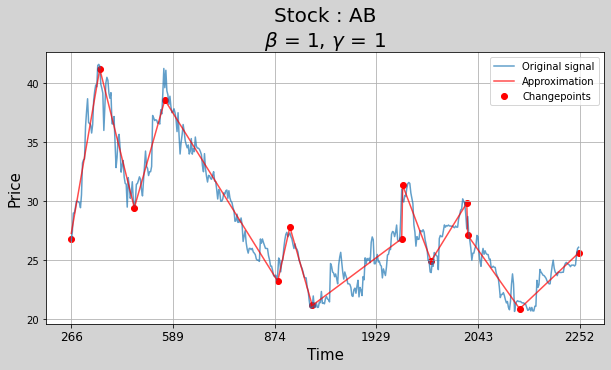
\includegraphics[width=0.495\textwidth]{figures/comparaison CPOP PELT/CPOP.png}
    \caption{Comparison of the PELT method (left) and the CPOP method (right) on the stock of the company "Amen Bank" (AB).}
    \label{fig:comparison}
\end{figure}

We see on figure \ref{fig:comparison} that the CPOP method is able to detect the changepoints much more accurately than the PELT method. More precisely, the PELT method exhibits a clear tendency to detect multiple changepoints between two consecutive CPOP changepoints. This is due to the fact that the PELT method is, by design, only able to detect changes in the mean of the signal; Therefore, along a steep trend, as the signal rapidly and monotonically varies, it will detect multiple changepoints, while the CPOP method will only detect one changepoint at the beginning of the trend and one at the end.

\subsection{Influence of the penalty parameter $\beta$}
Next, we investigate the influence of the penalty parameter $\beta$ on the number of changepoints detected. We see on figure \ref{fig:beta} that the number of changepoints detected is a decreasing function of $\beta$. This is consistent with the fact $\beta$ penalizes the number of changepoints.

\subsection{Influence of the segment cost $h$}

\subsection{Computational complexity}

\section{Appendix}
\end{document}
